\chapter[TP3]{\uline{TP3}}

On consid\`ere une carte g\'eographique mod\'elis\'ee par une fonction A d\'efinie sur le carr\'e [0, L] × [0, L]. La quantité A(x, y) d\'esigne
l’altitude du point (x, y). De l’eau peut s’ecouler sur cette topographie. La surface de l’eau se trouve \`a l’altitude A(x, y)+h(x, y, t).
La hauteur d’eau h ≥ 0 étant petite devant L, le champ de vitesse est quasi-horizontal et constant suivant z. La vitesse est enti\`erement d\'etermin\'ee par ses composantes suivant x et y u(x, y, t) et v(x, y, t). Par convention, on convient que la vitesse est
nulle sur une zone s\'eche, c’est \`a dire aux points (x, y, t) o\`u h(x, y, t) = 0. 


\section[R\`esolution num\'erique de l`\'equation de Saint-Venant en 2D]{\uline{R\`esolution num\'erique de l`\'equation de Saint-Venant en 2D:}}

Dans ce cadre, le mod\'ele de Saint-Venant (ou shallow water) s’ecrit:

\begin{equation}
\label{systeme}
\left \lbrace \begin{array}{rl}
\partial_t h +  \partial_x hu + \partial_y hv = 0, \\
\partial_t hu  +  \partial_x (h u^2 + g \frac{h^2}{2}) + \partial_y huv = -gh\partial_xA, \\
\partial_t hv  + \partial_x huv +  \partial_y (h v^2 + g \frac{h^2}{2})  = -gh\partial_xA, \\

\end{array}\right.
\end{equation} 

\subsection[R\'e\'ecrire le syst\`eme de Saint-Venant 2D]{\uline{R\'e\'ecrire le syst\`eme de Saint-Venant 2D:}}

On pose: $w = \begin{pmatrix}
h\\
hu \\
hv
\end{pmatrix}= \begin{pmatrix}
w_1\\
w_2 \\
w_3
\end{pmatrix}$

On a donc:

$F_1(w) = \begin{pmatrix}
w_2\\
\frac{w_2^2}{w_1} + g \frac{w_1^2}{2}\\
\frac{w_2 w_3} {w_1}
\end{pmatrix}=
\begin{pmatrix}
hu\\
h u^2 + g \frac{h^2}{2}\\
huv
\end{pmatrix}$
et:
$F_2(w) = \begin{pmatrix}
w_3\\
\frac{w_2 w_3} {w_1}\\
\frac{w_3^2}{w_1} + g \frac{w_1^2}{2}
\end{pmatrix}=
\begin{pmatrix}
hv\\
huv\\
h v^2 + g \frac{h^2}{2}
\end{pmatrix}$

avec
$S(w) = \begin{pmatrix}
0\\
-gw_1\partial_xA\\
-gw_1\partial_xA 
\end{pmatrix}$

Afin de r\'e\'ecrire le syst\`eme de Saint-Venant 2D:

$$\partial_t w +  \partial_x F_1(w) + \partial_y F_2(w) = S(w)$$


\subsection[Le syst\`eme de Saint-Venant 2D est hyperbolique?]{\uline{Le syst\`eme de Saint-Venant 2D est hyperbolique?:}}

pour montrer que le système est dit hyperbolique, on montre que $\partial_w F(w) · n$ est diagonalisable avec des valeurs propres r\'eelles pour tout w tel que $w_1 ≥ 0$ et pour tout n. En particulier, puisque le syst\`eme est sym\`etrique par rotation on prent $n = (1,0)$ alors il suffit de montrer que,
$\partial_w F_1(w)$ est diagonalisable avec des valeurs propres r\'eelles pour tout w.

En effet:

$$F'_1(w) = \begin{pmatrix}
0 & 1& 0\\
-\frac{w_2^2}{w_1^2} + g w_1 & 2 \frac{w_2}{w_1} & 0\\
-\frac{w_2 w_3} {w_1^2} & \frac{w_3} {w_1} & \frac{w_2} {w_1}
\end{pmatrix}$$

On calcule le polyn\^ome caract\'eristique:

$$det(F_1'(w) - \lambda I) = \begin{vmatrix}
-\lambda & 1& 0\\
-\frac{w_2^2}{w_1^2} + g w_1 & 2 \frac{w_2}{w_1} - \lambda & 0\\
-\frac{w_2 w_3} {w_1^2} & \frac{w_3} {w_1} & \frac{w_2} {w_1} - \lambda
\end{vmatrix} $$

$\implies$

$$det(F_1'(w) - \lambda I) = (\frac{w_2} {w_1} - \lambda) \big(-\lambda (2 \frac{w_2}{w_1} - \lambda) + \frac{w_2^2}{w_1^2} - g w_1 \big)$$

$\implies$

$$det(F_1'(w) - \lambda I) = (\frac{w_2}{w_1} - \lambda) \big((\lambda - \frac{w_2}{w_1})^2  - g w_1 \big)$$

$\implies$

$$det(F_1'(w) - \lambda I) = (\frac{w_2}{w_1} - \lambda) (\lambda - \frac{w_2}{w_1} + \sqrt{g w_1})(\lambda - \frac{w_2}{w_1} - \sqrt{g w_1})$$

en outre $det(F_1'(w) - \lambda I)$ $\implies$

$$\left \lbrace \begin{array}{rl}
\lambda_1 = \frac{w_2}{w_1} \\
\lambda_2 =  \frac{w_2}{w_1} + \sqrt{g w_1}\\
\lambda_3 =  \frac{w_2}{w_1} - \sqrt{g w_1}
\end{array}\right.$$

et donc pour toute direction:
$$\left \lbrace \begin{array}{rl}
\lambda_1 = \frac{w_2}{w_1}.n \\
\lambda_2 =  \frac{w_2}{w_1}.n + \sqrt{g w_1}\\
\lambda_3 =  \frac{w_2}{w_1}.n - \sqrt{g w_1}
\end{array}\right.$$

On remarque que les valeurs propres sont bien r\'eelles pour tout w et de multiplicit\'e 3 donc le syst\'eme est bien hyperbolique.

\subsection[Le flux num\'erique f(wL, wR, n) de Rusanov en 2D]{\uline{Le flux num\'erique f(wL, wR, n) de Rusanov en 2D:}}

On souhaite réaliser une approximation numérique du système de Saint-Venant au moyen de la méthode des volumes finis. pour ceci on explicite d'abord le flux numérique en l'occurrence celui de rusanov:

$$f(w_L,w_R,n) = \frac 1 2 \big(f(w_L,n)+ f(w_R,n)\big) - \frac{\lambda(w_L,w_R)}{2}(w_R-w_L)$$

avec le flux physique dans une direction n:
$$f(w,n) = f(w).n = F_1(w).n_1 + F_2(w).n_2 $$
o\`u les $\lambda_k$ sont les valeurs propres de $f'(w,n)$:

$$\lambda(w_L,w_R) = max_k max(|\lambda_k(w_L,n)|,|\lambda_k(w_R,n)|)$$

pour optimiser les calcules on fixe $\lambda$:
$$\lambda(w_L,w_R) = max(|\frac{w_2}{w_1}.n + \sqrt{g w_1}|_L,|\frac{w_2}{w_1}.n - \sqrt{g w_1}|_R)$$


\subsection[ D\'ecrire comment utiliser le solveur de Riemann 1D pour le calcul en 2D]{\uline{D\'ecrire comment utiliser le solveur de Riemann 1D pour le calcul en 2D:}}

On fait un changement de variable d\`crit ci-dessous qui ram\`ene le probl\`eme 2D en un probl\`eme 1D pour le r\'esoudre et en d\'eduire w.

\begin{lstlisting}

void flux_riem_2d(double *wL, double *wR, double *vnorm, double *flux)
{
    double qnL = wL [1] * vnorm [0] + wL [2] * vnorm [1];
    double qnR = wR [1] * vnorm [0] + wR [2] * vnorm [1];

    double qtL = -wL [1] * vnorm [1] + wL [2] * vnorm [0];
    double qtR = -wR [1] * vnorm [1] + wR [2] * vnorm [0];

    double vL [2] = {wL [0], qnL};
    double vR [2] = {wR [0], qnR};

    double v [2];
    double xi = 0;

    riem_stvenant (vL, vR, xi, v);

    double un = v [1] / v [0];
    double ut;

    ut = (un > 0) ? qtL / wL [0] : qtR / wR [0];

    double qn = v [1];
    double qt = ut * v [0];

    double w [3];
    w [0] = v [0];
    w [1] = qn * vnorm [0] - qt * vnorm [1];
    w [2] = qn * vnorm [1] + qt * vnorm [0];

    // puis calcul du flux physique (appliqué à w)
	fluxphy (w, vnorm, flux);
}
    
\end{lstlisting}


\subsection[Conditions aux limites: miroir, valeurs impos\'ees, zone s\`eche]{\uline{Conditions aux limites: miroir, valeurs impos\'ees, zone s\`eche:}}

\begin{itemize}
\item CL miroir:
Sur les bords les vitesse sont inv\'ers\'ee de sens:
$$w_m = \begin{pmatrix}
h\\
-hu \\
-hv
\end{pmatrix}
$$


\item CL impos\'ees:

On suvbstitue les valeurs impos\'ees:
$$w_i = \begin{pmatrix}
h\\
hu \\
hv
\end{pmatrix}$$

\item CL zone s\`eche:
Par convention, on convient que la vitesse est nulle sur une zone s\`eche, c’est \`a dire aux points (x, y, t) o\`u $h(x, y, t) = 0$.
donc:
$$w_s = \begin{pmatrix}
0\\
0 \\
0
\end{pmatrix}$$
\end{itemize}
\subsection[La r\'esolution du syt\`eme de Saint-Venant sur un maillage volume fini r\'egulier]{\uline{La r\'esolution du syt\`eme de Saint-Venant sur un maillage volume fini r\'egulier:}}



\subsection[Tester sur le cas 2D avec un fond plat]{\uline{Tester sur le cas 2D avec un fond plat:}}

pour diff\'erentes valeurs de T et avec un sch\'ema de Rusanov on obtient:
\begin{figure}[h!]
	\centering 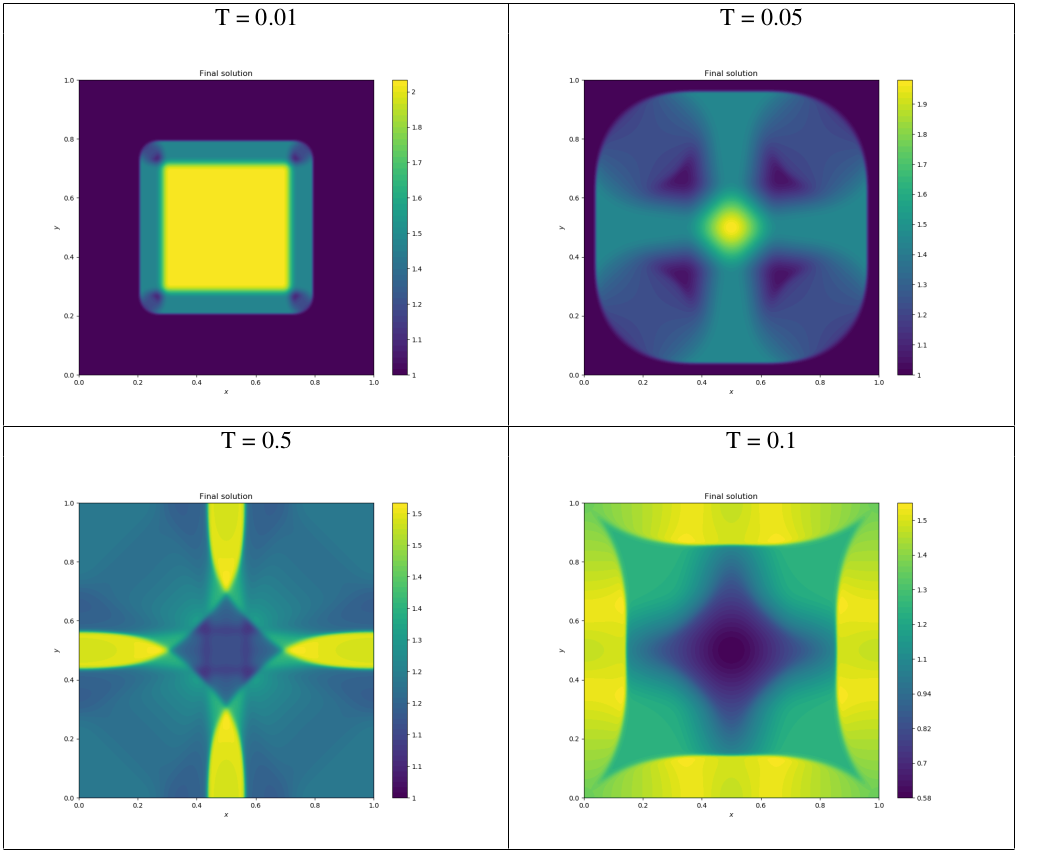
\includegraphics[scale=0.5]{Images_Fichiers/2D.png}
%\legend{template}
%\label{1CCG}
\end{figure}


\subsection[La correction MUSCL en 2D]{\uline{La correction MUSCL en 2D:}}

\subsection[Facultatif]{\uline{Facultatif:}}
















